\documentclass[12pt]{beamer}  
\usepackage{xeCJK}  
\usepackage{mathdots}  
\usepackage{graphicx}  
\usepackage{float}  
\usepackage{multirow}  
%\usepackage{cite}  
\usepackage{amsfonts, amsmath, mathrsfs, amsbsy, amssymb, dsfont,setspace}
\usepackage[square, comma, sort&compress, numbers]{natbib} 
\usepackage{algorithm}  
\usepackage{algorithmic} 
\usepackage{float} 
%\usetheme{Warsaw}  
\usetheme{CambridgeUS}
\begin{document} 
\title{低秩特性和联合稀疏的减弱墙体回波方法研究}  
\author{黄臣}  
\date{\today}  
\frame{\titlepage}  
\begin{frame}
  \frametitle{Low-Rank}
  如果$\bf X$是一个$m$行$n$列的数值矩阵,$\rm {rank(}\bf X\rm {)}$是$\bf X$的秩,
  假如$\rm {rank(}\bf X\rm {)}$远小于$m$和$n$,则我们称$\bf X$是低秩矩阵。
  秩可以度量相关性,当用少数几个线性无关的向量就可以表示整个矩阵时,说明矩阵
  具有低秩特性,在图像上,低秩特性表现为图像上的基底(字典)数目会很少。具体
  应用可以为拿来去除照片中的噪点,电影中的雨丝也可以通过低秩表达的方式来去除。

  而在穿墙雷达成像中,来自前墙的回波也被认为是具有低秩特性的矩阵,因此可以
  使用相关方法进行去除墙体回波。
\end{frame}
\begin{frame}
  \frametitle{Low-Rank}
  低秩矩阵逼近(LRMA)的方法被应用在很多地方,\citep{Ren2016Image}采用了一种
  加权核范数最小化的方法,用于先验盲图像去模糊。\citep{Tang2016Radar}则提
  出了一种迭代软阈值算法,用于使用减少的测量集来估计前墙回波的低秩矩阵和
  目标回波的稀疏矩阵。\citep{Bouzerdoum2017A}则是应用在了多极化信道的穿墙
  雷达成像上。
\end{frame}
\begin{frame}
  \frametitle{Soft thresholding algorithm}
  我们回波信号模型定为:
  \begin{equation} 
	\text{Z}=\text Z^{w}+\text{Z}^{t}+\Upsilon.
  \end{equation}
  所以我们的目标为估计$\text{Z}^w$和$\text{Z}^{t}$,这里采用鲁棒主成分分析
  (RPCA),所以优化问题描述为:
  \begin{equation} 
	\mathop{\text {minimize}}\limits_{\text{Z}^{w},\text{Z}^{t}} \Vert \text{Z}^{w}\Vert_{*}+\lambda\Vert \text{Z}^{t}\Vert_{1}\ \; \text{s.t}.\ \Vert \text{Z}-(\text{Z}^{w}+\text{Z}^{t})\Vert_{2} < \epsilon 
  \end{equation}
  当$\text{Z}$的全部数据被测量时,我们可以用凸优化的方法来解上式\citep{Chandrasekaran2009Rank}。 
\end{frame}
\begin{frame}
  \frametitle{Soft thresholding algorithm}
  在本例中,我们只测量了$K$个数据($K \ll N \times M$),记线性变换$\mathcal{A}$
  为$\mathbb{C}^{M\times\!N}\to\mathbb{C}^{K}$:
  \begin{equation*}
	\text{y}=\mathcal{A}(\text{Z})=\mathcal{A}(\text{Z}^{w}+\text{Z}^{t}+\Upsilon)
  \end{equation*}
  优化问题变为:
  \begin{equation}
	\mathop{\text{minimize}}\limits_{\text{Z}^{w},\text{Z}^{t}} \Vert \text{Z}^{w}\Vert_{*}+\lambda\Vert \text{Z}^{t}\Vert_{1}\ \text{s.t}.\ \Vert \text{y}-\mathcal{A}(\text{Z}^{w}+\text{Z}^{t})\Vert_{2} < \epsilon
  \end{equation}
  \citep{Waters2011SpaRCS}提出的SpaRSC贪婪算法,可用于解决该优化问题,但是需要
  有矩阵$\text{Z}$的稀疏水平的先验知识。
\end{frame}
\begin{frame}
  \frametitle{Soft thresholding algorithm}
  我们引入稀疏字典$\text{W}$来取代假设信号域的稀疏性,并将式(3)转化为拉格朗日
  正则化的形式:
  \begin{equation}
\mathop\text{minimize}\limits_{\text{Z}^{w},\text{Z}^{t}} \Vert \text{y}-\mathcal{A}(\text{Z}^{w}+\text{Z}^{t})\Vert_{2}+\lambda_{w}(\Vert \text{Z}^{w}\Vert_{*}+\lambda\Vert \text{WZ}^{t}\Vert_{1})
  \end{equation}
  为解决上面的问题,我们引入迭代软阈值的算法,使$\text{Z}^w$的奇异值和矩阵
  $\text{WZ}^t$的项收缩到0,阈值算子为:
  \begin{equation*}
	\mathcal{T}_{\tau}(x)=\frac{x}{\vert x\vert }(\vert x\vert -\tau)_{+}
  \end{equation*}
\end{frame}
\begin{frame}
  \frametitle{Soft thresholding algorithm}
  \scriptsize
  \begin{algorithm}[H]  
	\caption{软阈值迭代}
	\label{alg:1}
	\begin{algorithmic}[1]
	  \STATE{初始化:$\tilde{\text{Z}}_0=\mathcal{A}^Ty,\;\tilde{\text{Z}}_0^w=\tilde{\text{Z}_0},\; 
	  \tilde{\text{Z}}_0^t=0,\;i=1$}
	  \STATE{Step 1:$\tilde{\text{Z}}_{i}^{w}=\mathcal{S}_{\lambda_{w}}(\tilde{\text{Z}}_{i-1}-\tilde{\text{Z}}_{i-1}^{t})$}
	  \STATE{Step 2:$\tilde{\text{Z}}_{i}^{t}=\text{W}^{\dagger}(\mathcal{T}_{\lambda_{t}}\text{W}(\tilde{\text{Z}}_{i-1}-\tilde{\text{Z}}_{i-1}^{w}))$}
	  \IF{$\frac{\Vert\tilde{\text{Z}}_{i}^{w}+\tilde{\text{Z}}_{i}^{t}-(\tilde{\text{Z}}_{i-1}^{w}+\tilde{\text{Z}}_{i-1}^{t})\Vert_{2}}{\Vert\tilde{\text{Z}}_{i-1}^{w}+\tilde{\text{Z}}_{i-1}^{t}\Vert_{2}} < \delta $}
	  \STATE{结束}
	  \ELSE
	  \STATE{$\tilde{Z}_{i}=\tilde{\text{Z}}_{i}^{w}+\tilde{\text{Z}}_{i}^{t}-\mathcal{A}^{T}(\mathcal{A}(\tilde{\text{Z}}_{i}^{w}+\tilde{\text{Z}}_{i}^{t})-\text{y})$}
	  \STATE{$i\leftarrow i+1 $}
	  \STATE{回到Step 1}
	  \ENDIF
	\end{algorithmic}
  \end{algorithm}
\end{frame}
\begin{frame}{Multipolarization Through-wall Radar}
  回波信号模型和前面相似:
  \begin{equation}
	\text{Z}_l=\text Z^{w}_l+\text{Z}_l^{t}+\Upsilon_l
  \end{equation}
  其中$\text{Z}_l$表示第$l$个极化信道的回波。优化问题转化为:
  \begin{equation}
	\mathop{\text{minimize}}\limits_{\text{Z}^{w},\text{S}} \Vert \text{Z}^{w}\Vert_{*}+\lambda\Vert \text{S}^T\Vert_{2,1}\ \text{s.t}.\ \Big\Vert \text{Y}-\big[\mathcal{A}(\text{Z}^{w})+\Phi\Psi\text{S}\big]\Big\Vert_{F}^2 < \epsilon
  \end{equation}
  其中$\mathcal A(\text{Z}^w) = [\Phi\text{vec}(\text{Z}_1^w),\dots,\Phi\text{vec}(\text{Z}_L^w)] $,$\Phi$为稀疏字典,$\Psi\text S = \text Z^t$。
\end{frame}
\begin{frame}{Multipolarization Through-wall Radar}
  转化(6)为拉格朗日形式:
  \begin{equation}
	\frac{1}{2}\Big\Vert \text{Y}-\big[\mathcal{A}(\text{Z}^{w})+\Phi\Psi\text{S}\big]\Big\Vert_{F}^2 +\gamma\big(\Vert \text{Z}^{w}\Vert_{*}+\lambda\Vert \text{S}^T\Vert_{2,1}\big) 
  \end{equation}
  优化问题可分解为:
  \begin{equation}
	\begin{split}
  \text{Z}_{i+1}^w&=\mathop{\text{minimize}}\limits_{\text{Z}^{w}}\frac{1}{2}\Big\Vert \text{Z}_i-\text{Z}^{w}-\mathcal{A}^*(\Phi\Psi\text{S}_i)\Big\Vert_{F}^2 +\alpha\gamma\Vert\text{Z}^{w}\Vert_{*}\\ 
	\text{S}_{i+1}^w&=\mathop{\text{minimize}}\limits_{\text{s}}\frac{1}{2}\Big\Vert \text{Z}_{i}-\text{Z}^{w}_{i+1}-\mathcal{A}^*(\Phi\Psi\text{S})\Big\Vert_{F}^2 +\alpha\gamma\lambda\Vert\text{Z}^{w}\Vert_{*} 
  \end{split}
  \end{equation}

\end{frame}
\begin{frame}{Multipolarization Through-wall Radar}
\end{frame}
\begin{frame}{Multipolarization Through-wall Radar}
\end{frame}
\begin{frame}{Multipolarization Through-wall Radar}
\end{frame}
\begin{frame}{Multipolarization Through-wall Radar}
\end{frame}
\begin{frame}[allowframebreaks]{References}
  \footnotesize
  %\scriptsize
  \bibliographystyle{ieeetr} 
  \bibliography{ct.bib} 
\end{frame}
\end{document}
\begin{frame}
  \frametitle{Compressive Sensing Based Scene Reconstruction}
\end{frame}
\begin{frame}
  \frametitle{Compressive Sensing Based Scene Reconstruction}
\end{frame}
\begin{frame}
  \frametitle{Compressive Sensing Based Scene Reconstruction}
\end{frame}
\begin{frame}
  \frametitle{Compressive Sensing Based Scene Reconstruction}
\end{frame}
\*begin{figure}[H]
\centering
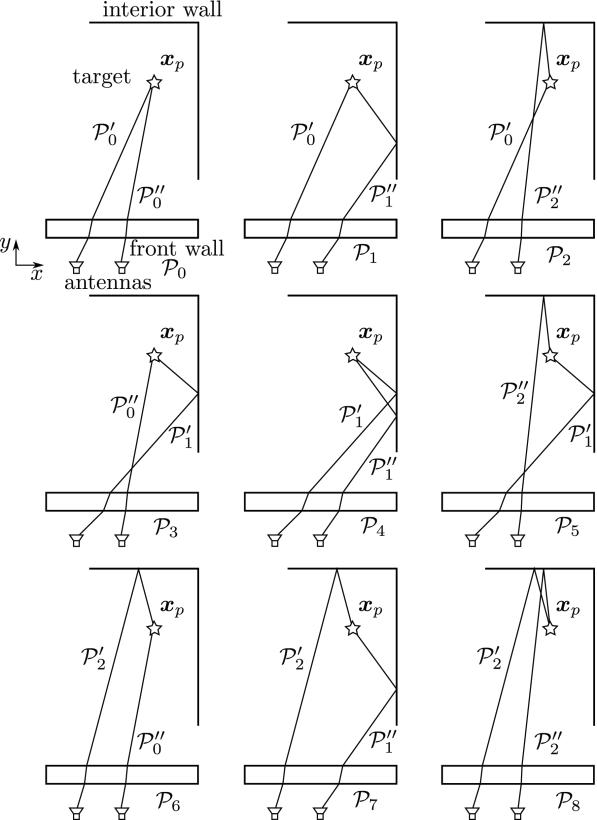
\includegraphics[width=0.5\textwidth]{fig2}
\caption{CSI处理流程图}
\end{figure}
